\documentclass[12pt,letterpaper]{article}

\usepackage{graphicx,amssymb,amsmath,bm,color,multicol}
\usepackage{../newcommand}
\sloppy
\newcommand{\ignore}[1]{}

\newenvironment{proof}{\noindent{\bf Proof:}}{\qed\bigskip}

\newtheorem{theorem}{Theorem}
\newtheorem{corollary}{Corollary}
\newtheorem{lemma}{Lemma} 
\newtheorem{claim}{Claim}
\newtheorem{fact}{Fact}
\newtheorem{definition}{Definition}
\newtheorem{assumption}{Assumption}
\newtheorem{observation}{Observation}
\newtheorem{example}{Example}
\newcommand{\qed}{\rule{7pt}{7pt}}

\newcommand{\homework}[4]{
	\thispagestyle{plain} 
	\newpage
	\setcounter{page}{1}
	\noindent
	\begin{center}
		\framebox{ \vbox{ \hbox to 6.28in
				{\bf ECON 4190: Industrial Organization \hfill #1} %change course name
				\vspace{4mm}
				\hbox to 6.28in
				{\hspace{2.5in}\large\mbox{Homework #2}}
				\vspace{4mm}
				\hbox to 6.28in
				{{\it Collaborators: #3\hfill}}
			}}
		\end{center}
	}

\oddsidemargin 0in
\evensidemargin 0in
\textwidth 6.5in
\topmargin -0.5in
\textheight 9.0in

\begin{document}

% Modify this command to be your name and computing ID
\homework{Fall 2021}{$3$}{Alex Shen (as5gd), Sean Velhagen (spv5hq), Max Bresticker (mtb9sex)}

Pledge: On my honor, I pledge that I have neither given nor received help on this assignment 
Signature: \textit{Alex Shen, Sean Velhagen, Max Bresticker}

\begin{enumerate}
	
\item

\begin{enumerate}
	\item Let $L$ refer to the left-wing candidate and $R$ refer to the right-wing candidate. Simply as a matter of their positions, $L$ will always receive the $\frac{1}{4}$ to their left, and $R$ will always receive the $\frac{1}{8}$ to their right. However, given a uniform distribution we only have to figure out $\hat{x}$, the location of the voter that is indifferent between the candidates, to determine the share each candidate receives.

	Given the general utility function $v_i = r_i - T | x-l_i |$, utilities for a voter for $L$ and $R$ can be determined to equal $v_L = r_1 - T(x - \frac{1}{4})$ and $v_R = r_2 - T(\frac{7}{8} - x)$ respectively. Now we simply solve for x when $v_L = v_R$:
	
	\begin{align*}
		v_L &= v_R \\
		r_1 - T(\hat{x} - \frac{1}{4}) &= r_2 - T(\frac{7}{8} - \hat{x}) \\
		2T(\hat{x}) &= r_1 - r_2 + \frac{9}{8}T \\
		\hat{x} &= \frac{r_1 - r_2}{2T} + \frac{9}{16}
	\end{align*}
	
	Therefore, $L$ will receive $\hat{x}$ of the vote, and $R$ will receive $1 - \hat{x}$ of the vote.

	\item Very similar process to before, simply change the function slightly.
	
	\begin{align*}
		r_1 - T(\hat{x} - \frac{1}{4})^2 &= r_2 - T(\frac{7}{8} - \hat{x})^2 \\
		&tl;dr \\
		r_1 - r_2 &= T(\hat{x} - \frac{1}{4})^2 - T(\hat{x} - \frac{7}{8})^2 \\
		\frac{r_1 - r_2}{T} &= \hat{x}^2 - \frac{\hat{x}}{2} + \frac{1}{16} - \hat{x}^2 + \frac{7}{4}\hat{x} - \frac{49}{64} \\
		\frac{r_1 - r_2}{T} + \frac{45}{64} &= \frac{5}{4} \hat{x} \\
		\hat{x} &= \frac{4}{5}(\frac{r_1-r_2}{T}) + \frac{9}{16}
		% 1 - \hat{x} &= \frac{r_2 - r_1}{2T}
	\end{align*}

	Again, $L$ will receive $\hat{x}$ of the vote, and $R$ will receive $1 - \hat{x}$ of the vote.

	\item Once again, we know that at the very least, $L$ will always receive the voters spanning the $\frac{1}{4}$ to their left, and $R$ will always receive the voters spannihg the $\frac{1}{8}$ to their right. Given the changed distribution, we know that they will each receive $\frac{1}{8}$ of the votes at least.
	
	To determine the rest, we need to determine how the votes in the middle are split. Thankfully, we already calculated the location of the indifferent voter $\hat{x}$ in part A to be $\frac{r_1 - r_2}{2T} + \frac{9}{16}$ which we can reuse here. From this, we can then calculate how many votes from the ``middle" each candidate gets by multiplying the ``distance" to the indifferent voter from each candidate by the voter density within that region, $\frac{3}{4} * \frac{1}{\frac{7}{8} - \frac{1}{4}} = \frac{6}{5}$. We know that each candidate also receives $\frac{1}{8}$ from their base, and also since there are only 2 candidates, the number of votes from either candidate can be determined once we know one. We solve for the votes gained by the left candidate as followed:

	\begin{align*}
		{votes}_L &= \frac{6}{5} (\hat{x} - \frac{1}{4}) + \frac{1}{8} \\
		% &tl;dr \\
		&= \frac{6}{5} (\frac{r_1-r_2}{2T} + \frac{9}{16} - \frac{1}{4}) + \frac{1}{8} \\
		&= \frac{6}{5} * \frac{r_1 - r_2}{2T} + \frac{6}{5} * \frac{5}{16} + \frac{1}{8} \\
		{votes}_L(T,r_1, r_2) &= \frac{6}{5} * \frac{r_1 - r_2}{2T} + \frac{1}{2} \\
		1 - {votes}_L = {votes}_R(T,r_1, r_2) &= \frac{3}{5} * \frac{r_2 - r_1}{T} + \frac{1}{2}
	\end{align*}

	\item Reusing a lot of our work from before, we know the density of the middle region is $\frac{1}{3}* \frac{1}{\frac{7}{8} - \frac{1}{4}} = \frac{8}{15}$
	
	\begin{align*}
		{votes}_L &= \frac{8}{15} (\frac{r_1 - r_2}{2T} + \frac{9}{16} - \frac{1}{4}) + \frac{1}{3} \\
		{votes}_L(T,r_1, r_2) &= \frac{4}{15} (\frac{r_1 - r_2}{T}) + \frac{1}{2} \\
		1 - {votes}_L  = {votes}_R(T,r_1, r_2) &= \frac{4}{15} (\frac{r_2 - r_1}{T}) + \frac{1}{2}
	\end{align*}

	The right candidate (who is further to the right than the left candidate is to the left) gets more votes here than in part C - this indicates that it's especially important for candidates positioned further from the center to have larger bases of support. 
\end{enumerate}

\item 

\begin{enumerate}
	\item To find $Q_i$, we first have to find the indifferent consumers between firm $i$ and firms $i-1$ and $i+1$, called $\hat{x}_L$ and $\hat{x}_R$. Using the utility equation $v_i = r - p_i - T | x - l_i |$, we can solve for both as follows:

\begin{align*}
	r - p_{i-1} - T(\hat{x}_L - \frac{i-1}{n}) &= r - p_i - T(\frac{i}{n} - \hat{x}_L) \\
	p_i - p_{i-1} &= T(\hat{x}_L - \frac{i-1}{n}) - T(\frac{i}{n} - \hat{x}_L) \\ 
	&= T\hat{x}_L - \frac{Ti-T}{n} - \frac{Ti}{n} + T\hat{x}_L \\
	&= 2T\hat{x}_L - \frac{2Ti - T}{n} \\
	2T\hat{x}_L &= p_i - p_{i-1} +  \frac{2Ti - T}{n} \\
	\hat{x}_L &= \frac{p_i - p_{i-1}}{2T} + \frac{2i - 1}{2n}
\end{align*}

\begin{align*}
	r - p_{i+1} - T(\frac{i+1}{n} - \hat{x}_R) &= r - p_i - T(\hat{x}_R - \frac{i}{n}) \\
	p_i - p_{i+1} &= T(\frac{i+1}{n} - \hat{x}_R) - T(\hat{x}_R - \frac{i}{n}) \\ 
	&= \frac{Ti+T}{n} - T\hat{x}_R - T\hat{x}_R + \frac{Ti}{n} \\
	&= \frac{2Ti + T}{n} - 2T\hat{x}_R \\
	2T\hat{x}_R &= p_{i+1} - p_i +  \frac{2Ti - T}{n} \\
	\hat{x}_R &= \frac{p_{i+1} - p_i}{2T} + \frac{2i + 1}{2n}
\end{align*}

Finding the difference $\hat{x}_R$ and $\hat{x}_L$ gives us the share of the market firm $i$ sells to, and since $M=1$, also gives us the demand $Q$:

\begin{align*}
	Q &= \hat{x}_R - \hat{x}_L = \frac{p_{i+1} - p_i}{2T} + \frac{2i + 1}{2n} - (\frac{p_i - p_{i-1}}{2T} + \frac{2i - 1}{2n}) \\
	&\therefore Q_i (p_i, p_{i-1}, p_{i+1} )  = \frac{p_{i+1} - 2p_i + p_{i-1}}{2T} + \frac{1}{n}
\end{align*}

\item If $p_{i-1} = p_{i+1} = p$ then our derived $Q_i$ reduces to  $\frac{p-p_i}{T} + \frac{1}{n}$.

\item To find CS, we need to find the area as shown in this graph:

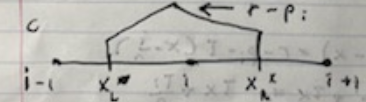
\includegraphics{2c.PNG}

Doing so requires finding $v(\hat{x}_L)$ and $v(\hat{x}_R)$, the utility gained by the indifferent consumers on both ends of firm $i$. Given that all non-$i$ firms are charging the same price, we know that the problem must be symmetrical, so we only need to solve for $v(\hat{x}_L)$. \textit{Note: the problem has some ambiguity in its wording regarding whether or not the assumption from part B that all firms except $i$ are charging the same price $p$ still holds. Since it makes the computation simpler, and the problem was presented during discussion as having this assumption, we have also made this assumption here.}

\begin{align*}
	v(\hat{x}_L) &= r - p_i - T(\frac{i}{n} - (\frac{p_i - p}{2T} + \frac{2i - 1}{2n})) \\
	&= r - p_i - \frac{Ti}{n} + \frac{p_i - p}{2} + \frac{Ti}{n} - \frac{T}{2n} \\
	v(\hat{x}_L) = v(\hat{x}_R) &= r - p_i + \frac{p_i - p}{2} - \frac{T}{2n}
\end{align*}

This gives us everything we need to solve for consumer surplus:

\begin{align*}
	CS &= v(\hat{x}_L) * Q + \frac{1}{2} (r-p_i - v(\hat{x}_L)) * Q = Q (v(\hat{x}_L) * Q + \frac{1}{2} (r-p_i - v(\hat{x}_L))) \\
	CS &= (\frac{p-p_i}{T} + \frac{1}{n}) * [(r - p_i + \frac{p_i - p}{2} - \frac{T}{2n}) + \frac{1}{2} (r - p_i - (r - p_i + \frac{p_i - p}{2} - \frac{T}{2n})] \\
	CS &= (\frac{p-p_i}{T} + \frac{1}{n}) * [(r - p_i + \frac{p_i - p}{2} - \frac{T}{2n}) + \frac{1}{2} (\frac{T}{2n} - \frac{p_i - p}{2})]
\end{align*}

\item Setting $p_i = p$ greatly simplifies our equation, which we can also then simply multiply by $n$ firms to find total consumer surplus in the city:

\begin{align*}
	CS_i &= (\frac{p-p}{T} + \frac{1}{n}) * [(r - p + \frac{p - p}{2} - \frac{T}{2n}) + \frac{1}{2} (\frac{T}{2n} - \frac{p - p}{2})] \\ 
	CS_i &= \frac{1}{n} * [r - p - \frac{T}{2n} + \frac{T}{4n}] \\
	CS_{city} &= n * CS_i = r - p - \frac{T}{2n} + \frac{T}{4n}
\end{align*}
\end{enumerate}
\end{enumerate}
	
\end{document}
